\documentclass[usenatbib,usegraphicx,letterpaper]{mn2e}
\usepackage[totalwidth=480pt,totalheight=680pt]{geometry}

\usepackage{amssymb}
\usepackage{epsfig}
\usepackage{amsmath}
\usepackage{color}
%\usepackage{hyperref}

\bibliographystyle{mn2e} 

%-------- journals
\newcommand{\araa}{ARAA~}
\newcommand{\apj}{ApJ~}
\newcommand{\apjl}{ApJL~}
\newcommand{\apjs}{ApJS~}
\newcommand{\mnras}{MNRAS~}
\newcommand{\nat}{Nature~}
\newcommand{\physrep}{Phys. Rep.~}
\newcommand{\aj}{AJ~}
\newcommand{\pasp}{ASP~}

%%%% Misc %%%
\newcommand{\beq}{\begin{equation}}
\newcommand{\eeq}{\end{equation}}
\newcommand{\beqray}{\begin{eqnarray}}
\newcommand{\eeqray}{\end{eqnarray}}

\newcommand{\ben}{\begin{enumerate}}
\newcommand{\een}{\end{enumerate}}
\newcommand{\bit}{\begin{itemize}}
\newcommand{\eit}{\end{itemize}}

%%%%%%%%  galaxy properties  %%%%%%%%
\newcommand{\rhalf}{R_{1/2}}
\newcommand{\rhalfdisk}{R_{1/2}^{\rm disk}}
\newcommand{\rhalfbulge}{R_{1/2}^{\rm bulge}}
\newcommand{\adisk}{A_{\rm disk}}
\newcommand{\abulge}{A_{\rm bulge}}
\newcommand{\alphadisk}{\alpha_{\rm disk}}
\newcommand{\alphabulge}{\alpha_{\rm bulge}}
\newcommand{\sigmarhalf}{\sigma_{\rm R_{1/2}}}
\newcommand{\rvir}{R_{\rm vir}}
\newcommand{\bt}{{\rm B/T}}
\newcommand{\mstar}{M_{\ast}}
\newcommand{\ssfr}{{\rm sSFR}}
\newcommand{\sfr}{{\rm SFR}}

%%%%%%%%  halo properties  %%%%%%%%
\newcommand{\halospin}{\lambda_{\rm halo}}
\newcommand{\mvir}{M_{\rm vir}}
\newcommand{\macc}{M_{\rm acc}}
\newcommand{\mpeak}{M_{\rm peak}}
\newcommand{\mhalo}{M_{\rm halo}}


%%%%%%%%  observations  %%%%%%%%
\newcommand{\rproj}{r_{\rm p}}
\newcommand{\wproj}{w_{\rm p}}

%%%%%%%%  units  %%%%%%%%
\newcommand{\kpc}{{\rm kpc}}
\newcommand{\mpc}{{\rm Mpc}}

%%%%%%%%%%%%%%%%%%%%%%%%%%%%%%%%
%%%%%%%%%%%%%%%%%%%%%%%%%%%%%%%%


\usepackage{epsfig}  \usepackage{graphicx}   \usepackage{rotating}

\begin{document}

\title[The Galaxy Size--Halo Connection]
{Galaxy Clustering Constraints on the Galaxy Size--Halo Connection}


\author[Hearin, Behroozi, Kravtsov \& Moster]{
Andrew Hearin$^{1}$, Peter Behroozi$^{2}$, Andrey Kravtsov$^{3}$, Benjamin Moster$^{4}$\\
$^{1}$Argonne National Laboratory, Argonne, IL, USA 60439, USA\\
$^{2}$Department of Physics, University of Arizona, 1118 E 4th St, Tucson, AZ 85721 USA\\
$^{3}$Department of Astronomy \& Astrophysics, The University of Chicago, Chicago, IL 60637 USA\\
$^{4}$Universit{\"a}ts-Sternwarte, Ludwig-Maximilians-Universit{\"a}t M{\"u}nchen, Scheinerstr. 1, 81679 M{\"u}nchen, Germany
}

\maketitle

\begin{abstract}
We derive empirical modeling constraints on the connection between dark matter halos and the half-mass radius $\rhalf$ of galaxy bulges and disks. We show that both $\rhalfdisk$ and $\rhalfbulge$ are well-described by power law scaling relations with halo virial radius, $\rhalf=A\rvir^{\alpha}.$ Novel to this work, we use new SDSS measurements of the $\rhalf-$dependence of galaxy clustering to constrain the model parameters, $A_{\rm bulge}, A_{\rm disk}, \alpha_{\rm bulge},\alpha_{\rm disk},$ and log-normal scatter $\sigmarhalf.$ Even when only coarsely tuning these parameters to the observed one-point functions $\langle\rhalfdisk|\mstar^{\rm disk}\rangle$ and $\langle\rhalfbulge|\mstar^{\rm bulge}\rangle,$ our model accurately predicts the observed two-point clustering on small- and large-scales. This success non-trivial, as we show that galaxy clustering is highly sensitive to the physics that shapes satellite galaxy profiles. We find no evidence for the commonly assumed relation between halo spin $\halospin$ and $\rhalfdisk,$ and show that this assumption cannot be meaningfully constrained with either the clustering or lensing of  $L_{\ast}$ galaxies. Our results provide simple boundary conditions for more complex and fine-grained models of galaxy size. We make our python code publicly available to support cosmological surveys that require realistic synthetic galaxy populations.
\end{abstract}

\section{Introduction}
\label{sec:intro}
Some introduction goes here.

\section{Data and Simulations}
\label{sec:data}

\subsection{Galaxy Sample and Measurements}
\label{subsec:galaxydata}


Our galaxy sample comes from Data Release 10 of the Sloan Digital Sky Survey \citep[SDSS][]{ahn_etal14}. We study the same $\mstar-$complete galaxy sample used in \citet{behroozi_etal15}, to which we refer the reader for details. Values for $\mstar$ and $\sfr$ are taken from the MPA-JHU value-added catalog \citep{kauffmann_etal03,brinchmann_etal04}. 

We additionally use the catalog of SDSS galaxy profile decompositions provided by \citet{meert_etal15}. In the version of this catalog that we use, two-dimensional $r-$band profiles were fit with a two-component de Vaucouleurs + exponential profile for the bulge and disk, respectively. We cross-match our DR10 sample against the \citet{meert_etal15} scale radius of the composite profile, $\rhalf,$ and the $r-$band flux ratio of the two components, $\bt,$ giving us a volume-limited galaxy sample with values of $\mstar,\ssfr,\rhalf,$ and $\bt.$ 

We calculate two-point clustering $\wproj$ with line-of-sight projection of $\pi_{\rm max}=20\mpc$ using the {\tt correl} program in {\tt UniverseMachine}. Our results in \S~\ref{sec:results} will give special focus on the dependence of $\wproj$ upon composite galaxy size $\rhalf.$ We will quantify this dependence in terms of {\em clustering ratios} of ``large" vs. ``small" galaxies, defined according to whether composite galaxy size is above or below $\langle\rhalf\vert\mstar\rangle,$ computed as the median of a sliding stellar mass window with a width of $N_{\rm gal}=1000.$ 

Together with the present work, we make publicly available this cross-matched catalog, as well as code to generate the catalog from the original data files and load it into a python interpreter. 

\subsection{Simulation and Halos}
\label{subsec:sim}

{\tt Rockstar} subhalos identified at $z=0$ in the Bolshoi-Planck simulation are the basis of all our modeling. 

\subsection{Baseline Mock Catalog}
\label{subsec:baselinemock}

\subsubsection{Mapping $\mstar$ \& $\sfr$ to halos}
\label{subsubsec:umachine}

The starting point of our model is the best-fit {\tt UniverseMachine} model \citep[][in prep]{behroozi_etal17}. This model maps stellar mass and star-formation rate to every halo and subhalo at each snapshot in the Bolshoi-Planck simulation. The stellar mass function, quenched fraction, SFR density, and SFR-dependent clustering are all accurately captured by this model from $z=0-10.$ The model we have developed in the present work does not depend in an essential way upon the {\tt UniverseMachine} model in particular, we only require some reasonably accurate starting point for the $\mstar$ and $\ssfr$ values mapped to simulated halos. 

\subsubsection{Mapping $\bt$ to halos}
\label{subsubsec:random_bt_model}

Our model for galaxy size is further predicated upon the mapping between dark matter halos and $\bt,$ the fraction of stellar mass in the bulge. In a companion paper to this work, we will present a separate empirical model for the $\bt-$halo connection. For our present purposes, we instead rely upon the simplest possible assumption for this connection that recovers the observed distribution $P(\bt\vert\mstar,\ssfr):$ we suppose that galaxy $\bt$ has no dependence whatsoever upon halo environment or assembly, beyond what is inherited by the mutual correlation between $\mstar, \ssfr$ and the cosmic web. That is, we map $\bt$ to dark matter halos by using the $\mstar$ and $\ssfr$ values from {\tt UniverseMachine} to randomly select the $\bt$ of a galaxy from our SDSS sample with a similar $\mstar$ and $\ssfr.$ The intuitive interpretation of this modeling choice is that we assume the morphology-density relation is entirely determined by the color-density relation. 

\section{Galaxy Profile Model}
\label{sec:model}

Motivated by the \citet{kravtsov13} results, we model the half-mass radii of galaxies as separate power law functions of halo virial radius:

\begin{eqnarray}
\label{eq:fiducial_model}
\rhalfbulge &=& \abulge\rvir^{\alphabulge} \\
\rhalfdisk &=& \adisk\rvir^{\alphadisk} 
\end{eqnarray}

For central galaxies residing in host halos, we use the present-day virial radius; for satellite galaxies we use the virial radius at the time of accretion, using physical units of $\kpc.$ We model the composite size of model galaxies as 
\beq
\rhalf = (\bt)\rhalfbulge + (1-\bt)\rhalfdisk.
\eeq

When generating Monte Carlo realizations of our model galaxy population, we add log-normal scatter $\sigmarhalf$ separately to each component. Our model for sizes thus has five free parameters: $\abulge, \adisk, \alphabulge, \alphadisk,$ and $\sigmarhalf.$ 

We reiterate an important distinction drawn in the formulation of our forward modeling approach. In the model described above, $\rhalfbulge$ and $\rhalfdisk$ are forward modeling quantities that we aim to constrain through SDSS observations of {\em composite} galaxy size $\rhalf.$ In particular, both model and real galaxies will be categorized as ``small" or ``large`` according to whether $\rhalf$ is above or below the median size for a galaxy with total stellar mass $\mstar.$

\section{Results}
\label{sec:results}

In \S~\ref{subsec:tests1} we show comparisons between the fiducial galaxy profile model described in \S~\ref{sec:model} and our SDSS sample. We demonstrate the sensitivity of galaxy clustering measurements to the post-infall evolution of satellite profiles in \S~\ref{subsec:tests2}, establishing the success of our fiducial model as non-trivial. In \S~\ref{subsec:tests3} we show that even highly idealized measurements of galaxy clustering and lensing are insensitive to assumptions about the relation between halo spin $\halospin$ and size $\rhalf$ of disk-dominated galaxies, implying that large-scale structure observations yield little-to-no constraining power on such assumptions. 

\subsection{Tests of the Fiducial Power Law Model}
\label{subsec:tests1}

\subsubsection{Scaling of $\rhalf$ with $\mstar$}
\label{subsubsec:scaling_relation}

In Figure \ref{fig:scatter_plot} we show the scaling of composite galaxy size $\rhalf$ with $\mstar,$ with separate panels dedicated to subsamples of galaxies divided according to value of $\bt.$ We refer to galaxies with $\bt<0.25$ as ``disk-dominated", $\bt>=0.75$ as ``bulge-dominated", and $0.25<=\bt<0.75$ as ``mixed morphology". 

The results shown in \citet{kravtsov13} simplify our task of parameter space exploration: the assumption that composite galaxy size $\rhalf$ scales in linear proportion to halo radius $\rvir$ gives a qualitatively good description of SDSS data over many orders of magnitude in galaxy mass. As first pointed out in \citet{kravtsov13}, this linearization is non-trivial because of the well-known curvature in the scaling relation of $\langle\rhalf\vert\mstar\rangle,$ which is visually apparent in all panels of Fig.~\ref{fig:scatter_plot}. 

Comparison of the top panels of Fig.~\ref{fig:scatter_plot} show that this linearization is only approximate; evidently, the composite size $\rhalf$ of bulge-dominated galaxies has a steeper scaling relation with $\mstar$ relative to disk-dominated galaxies. This difference motivates our simple extension of the \citet{kravtsov13} model, in which composite size $\rhalf$ of disk- and bulge-dominated galaxies scale according to separate power laws. 

Through MCMC parameter space exploration aided by {\tt emcee} \citep{emcee_hammer}, we find a good description of the observed one-point scaling relations is given by model galaxies with the parameters $\adisk=0.014=7\abulge, \alphadisk=1, \alphabulge=5/4,$ with log-normal scatter of $0.2$ dex motivated by \citet{somerville_etal17}. The black curves in Fig.~\ref{fig:scatter_plot} illustrate the median $\langle\rhalf\vert\mstar\rangle.$ 

We confirm the visual impression of comparing the top panels of Fig.~\ref{fig:scatter_plot}: we are unable to find a parameter combination in which the composite size of both bulge- and disk-dominated galaxies have linear ($\alpha=1$) scaling with $\rvir.$ We do not quantitatively rule out such a scaling relation, as this would require careful investigation of the systematic error budget of galaxy profile modeling that we consider beyond the scope, though well-motivated, by the present work. 
 
\subsubsection{Dependence of clustering on $\rhalf$}
\label{subsubsec:clustering_tests}

\subsection{Sensitivity of Clustering to Satellite Profile Evolution}
\label{subsec:tests2}


\subsection{Insensitivity of Clustering and Lensing to Halo Spin Correlations}
\label{subsec:tests3}

%---------------------------------------------------------------------------------------------------
\begin{figure*}
\centering
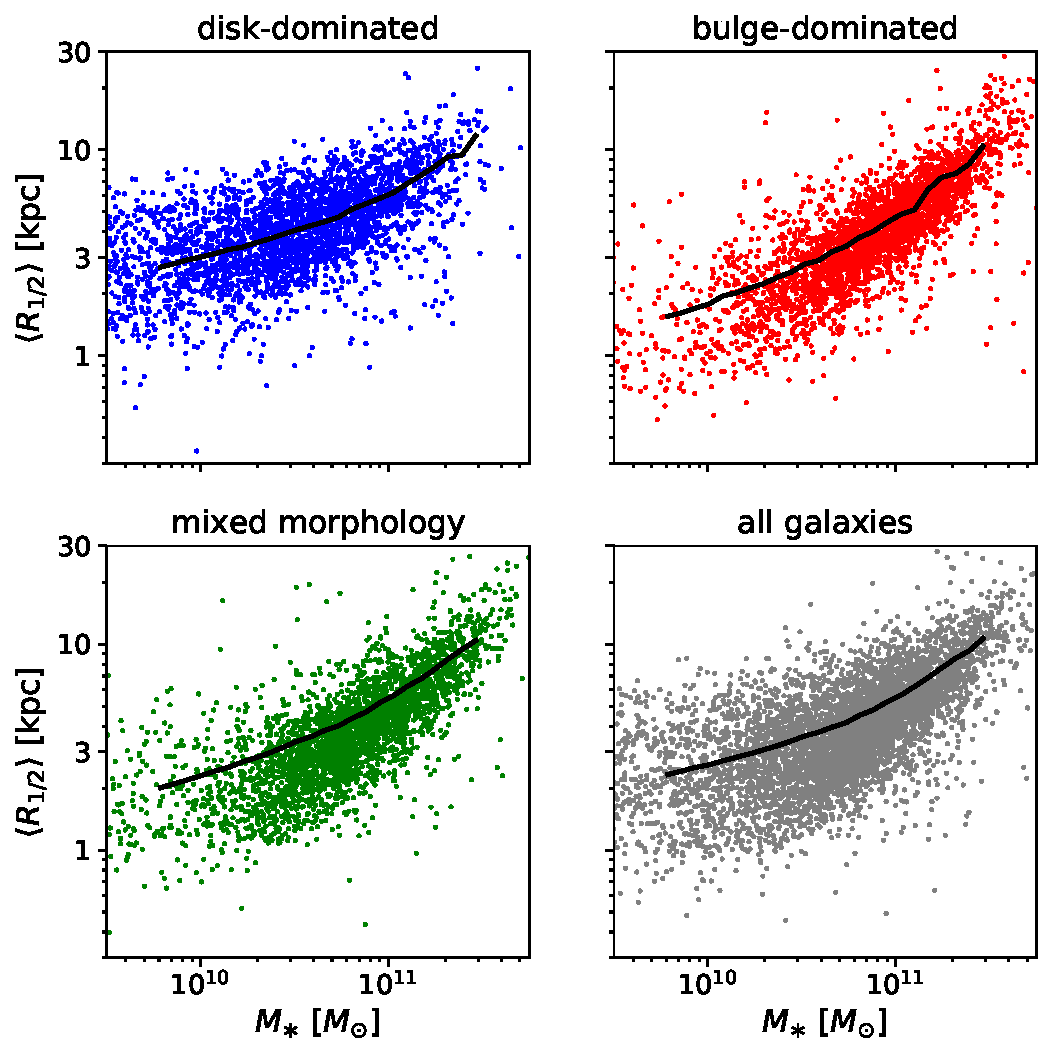
\includegraphics[width=12cm]{FIGS/size_vs_stellar_mass_multipanel_bt_decomposition.pdf}
\caption{
{\bf One-point data used to fit the fiducial model.}
Scattered points show the $\rhalf-\mstar$ relation for SDSS galaxies as measured in \citet{meert_etal15}. Bulge-dominated galaxies are defined in terms of the bulge-to-total stellar mass ratio $\bt>=0.75,$ disk-dominated galaxies $\bt<0.25,$ mixed morphology as $0.25 < \bt < 0.75.$ The black curve in each panel shows the $\rhalf-\mstar$ relation implied by our fiducial model, in which $\rhalf=A\rvir^\alpha,$ with $\adisk=0.014=7\abulge, \alphadisk=1, \alphabulge=5/4,$ and uncorrelated log-normal scatter of $0.2$ dex about these relations. 
}
\label{fig:scatter_plot}
\end{figure*}
%-----------------------------------------------------------------------------------------------------

%---------------------------------------------------------------------------------------------------
\begin{figure*}
\centering
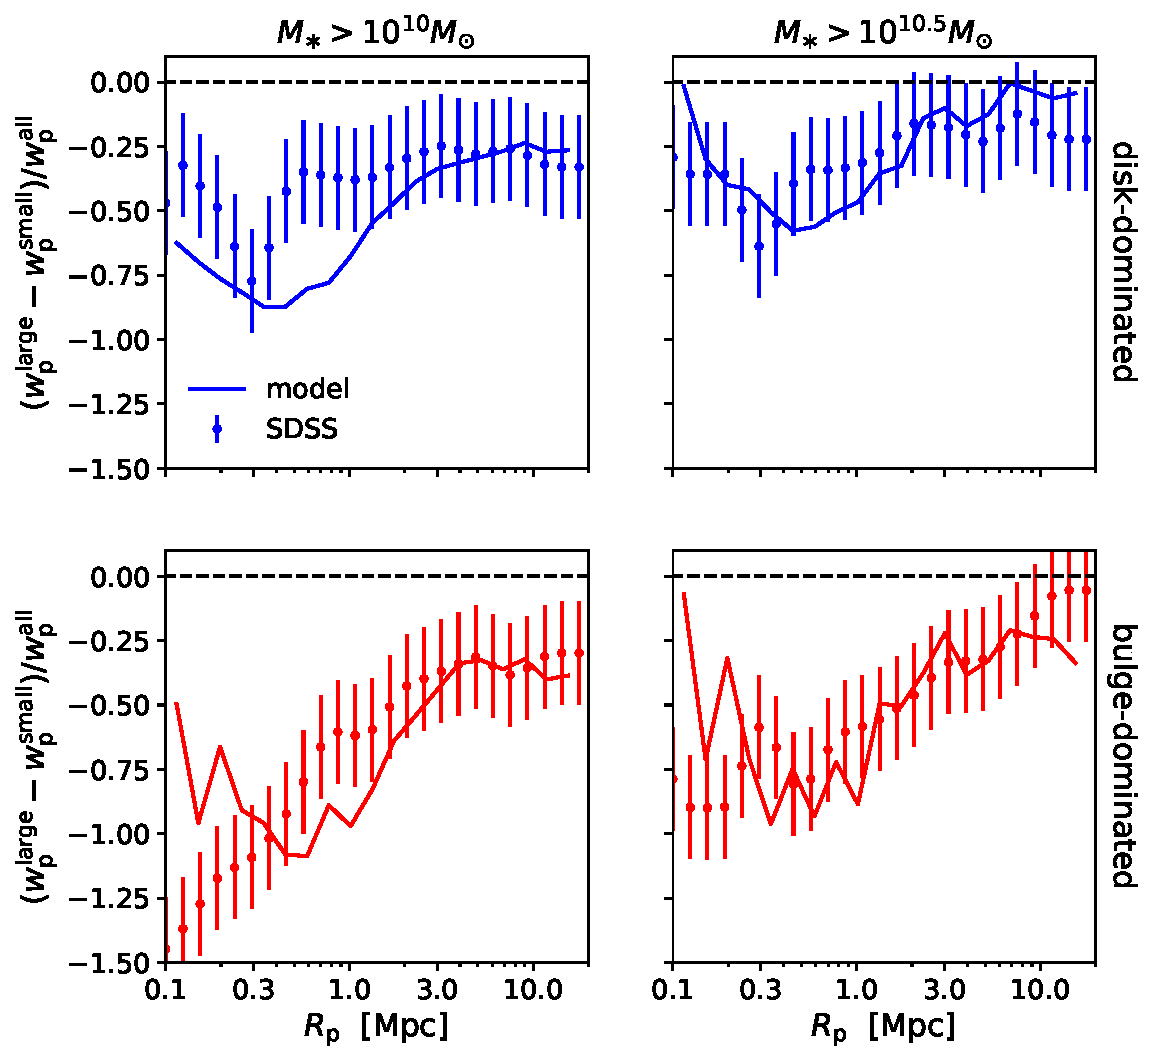
\includegraphics[width=12cm]{FIGS/size_clustering_ratios_bt_decomposition_model_vs_sdss.pdf}
\caption{
{\bf Two-point clustering data used to validate the fiducial model.}
Points with error bars show new SDSS measurements of the $\rhalf-$dependence of projected galaxy clustering, $\wproj,$ compared to predictions by the model tuned to the measurements shown in Fig.~\ref{fig:scatter_plot}. We define a disk or bulge as ``large" or ``small" according to whether it is above or below the median size for its stellar mass. The y-axis shows clustering strength ratios, so that, for example, a y-axis value of $-0.5$ corresponds to small galaxies being $50\%$ more strongly clustered than large galaxies of comparable stellar mass. We show results separately for disk-dominated galaxies ({\em top} panels) and bulge-dominated galaxies ({\em bottom }panels), and different thresholds in total stellar mass in the {\em left} and {\em right} panels. The successful prediction shown here is remarkable because the model was not fit to these data, and because two-point clustering is highly sensitive to the physics that shapes satellite galaxy profiles (see Fig.~\ref{fig:satellites}). 
}
\label{fig:clustering_ratio_upshot}
\end{figure*}
%-----------------------------------------------------------------------------------------------------

%---------------------------------------------------------------------------------------------------
\begin{figure}
\centering
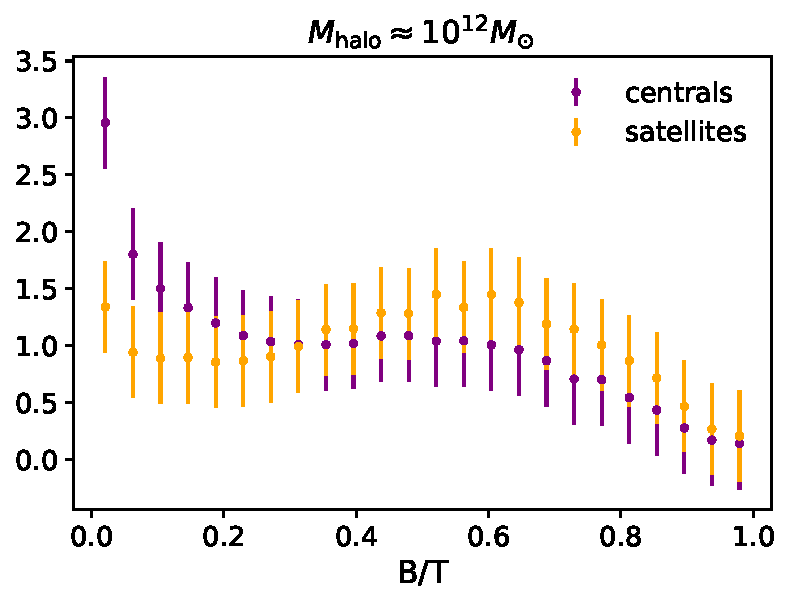
\includegraphics[width=8cm]{FIGS/random_bt_centrals_vs_satellites.pdf}
\caption{
{\bf Morphologies of centrals and satellites of the same halo mass.} We show the PDF of the bulge-to-total stellar mass ratio $\bt$ of central and satellite galaxies of the same halo mass $\mhalo=\mpeak.$ In the model, the PDF of $\bt$ is determined by the stellar mass $\mstar$ and specific star-formation rate $\ssfr$ statistically determine, with no residual dependence on the cosmic web. Satellite galaxies in the model are ``bulgier" than centrals of the same halo mass because satellites are more quiescent than centrals of the same stellar mass. Thus our baseline model ansatz is that the morphology-density relation is purely derived from the color-density relation. Since composite size $\rhalf$ in the model is given by $\rhalf=(\bt)\rhalfbulge + (1-\bt)\rhalfdisk,$ this ansatz in turn implies that smaller galaxies cluster more strongly relative to larger galaxies of the same stellar mass, as seen in the measurements shown in Fig.~\ref{fig:clustering_ratio_upshot}. 
}
\label{fig:bt_censat}
\end{figure}
%-----------------------------------------------------------------------------------------------------



%---------------------------------------------------------------------------------------------------
\begin{figure*}
\centering
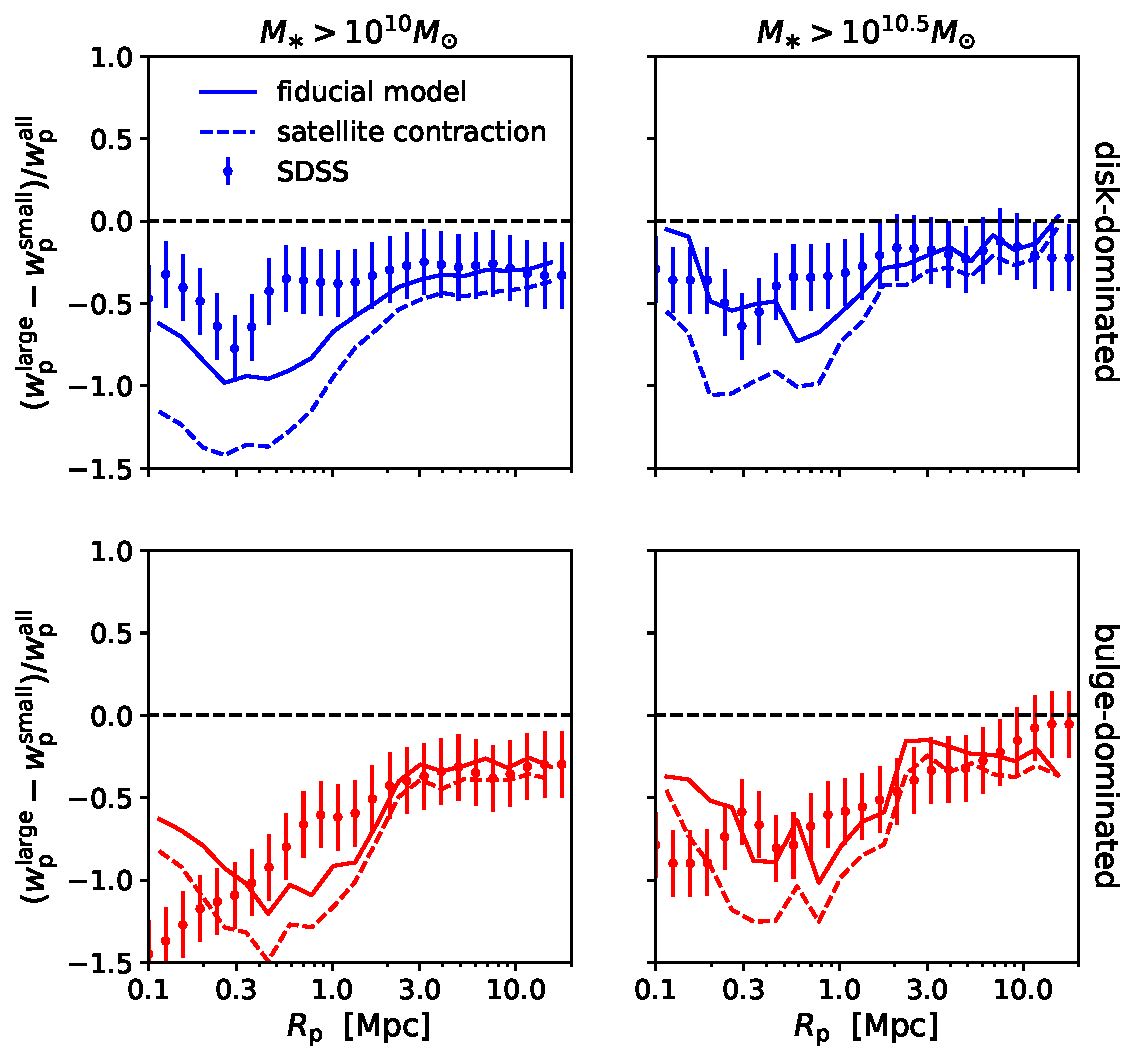
\includegraphics[width=12cm]{FIGS/alternate_satellite_models_size_clustering_ratios.pdf}
\caption{
{\bf Clustering provides tight constraints on the relative sizes of centrals and satellites.} 
Here we compare our fiducial model, in which satellite galaxy size is set by $\rvir$ at the time of infall, to an alternative model analogous to \citet{watson_etal12} in which satellite sizes contract in proportion to $(\mvir/\macc)^{1/3}.$ The large differences between solid and dashed curves in the top panels show that the $\rhalf-$dependence of galaxy clustering ratios is highly sensitive to the post-infall evolution of satellite galaxy profiles. The successful prediction of our fiducial model, in which satellite galaxies neither contract nor puff up after infall, places tight constraints on satellite-specific physical processes, which must be either negligible or conspiratorially produce little-to-no size change after accretion. 
}
\label{fig:satellites}
\end{figure*}
%-----------------------------------------------------------------------------------------------------


%---------------------------------------------------------------------------------------------------
\begin{figure*}
\centering
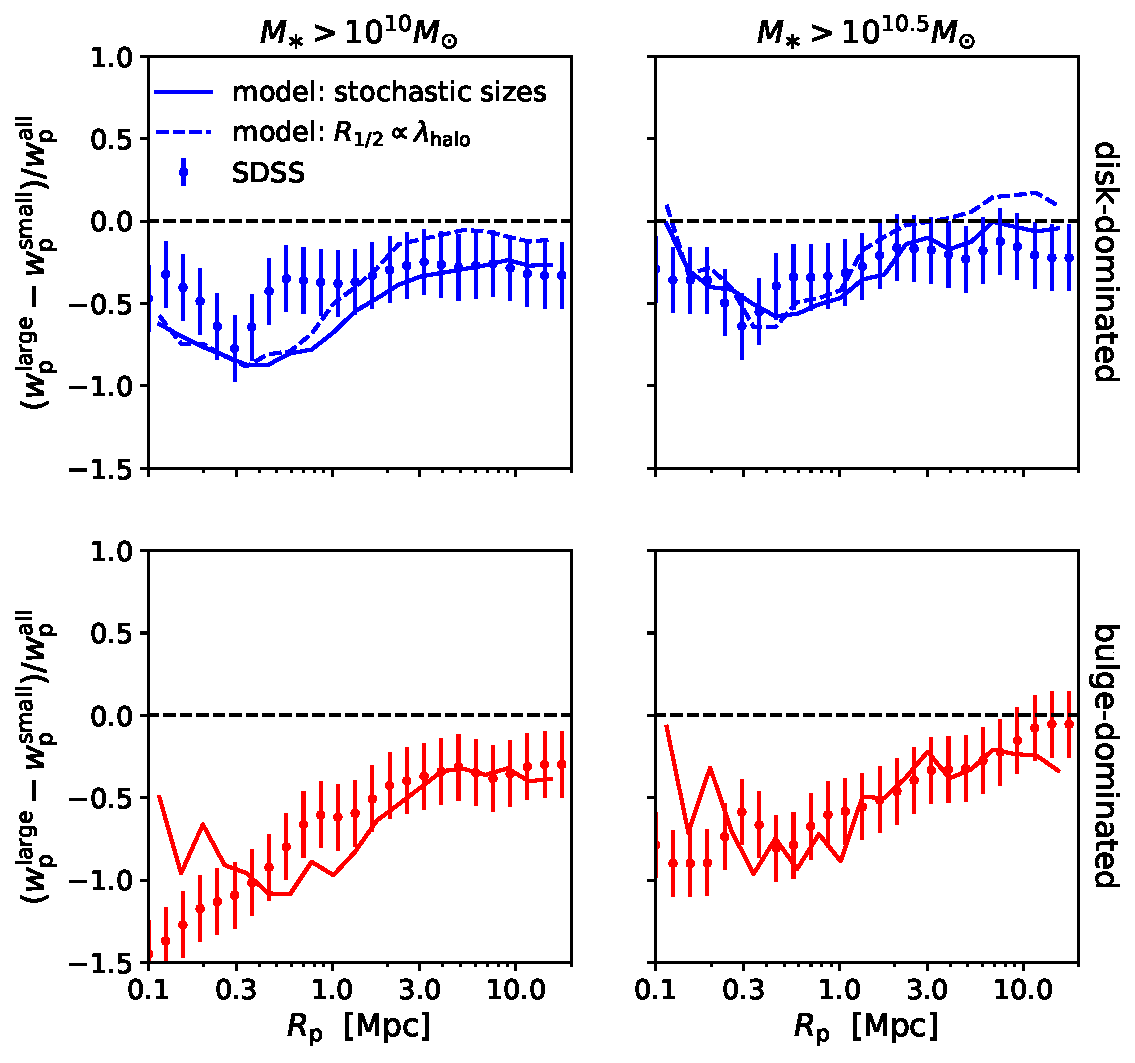
\includegraphics[width=8cm]{FIGS/size_clustering_ratios_bt_decomposition_spin_size_correlation.pdf}
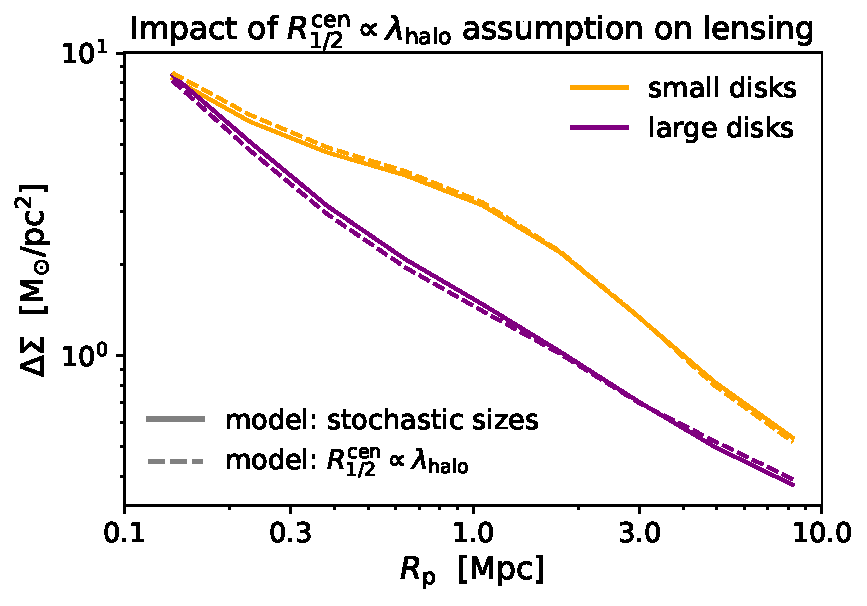
\includegraphics[width=8cm]{FIGS/central_lensing_spin_size_correlation.pdf}
\caption{
{\bf Clustering and lensing provide no constraining power on the assumption that $\rhalfdisk\propto\halospin.$} 
We compare the predictions between our fiducial model in which sizes are purely stochastic, and an alternative model motivated by \citet{mo_mao_white98} in which central galaxy disk size is maximally correlated with host halo spin at fixed stellar mass \citep[implemented via conditional abundance matching, e.g.,][]{hearin_etal13b}. The tiny differences between the solid and dashed curves imply that conventional large-scale structure measurements cannot even in principle provide compelling evidence pertaining to the assumption that $\rhalfdisk\propto\halospin.$ 
}
\label{fig:halospin_lensing}
\end{figure*}
%-----------------------------------------------------------------------------------------------------

\section{Discussion}
\label{sec:discussion}


\subsection{Progression from Backwards to Forwards Modeling}
\label{subsec:forwardsmodeling}

\subsection{Relation to Previous Work}
\label{subsec:previouswork}


\section{Conclusion}
\label{sec:conclusion}

\subsection{Summary}
\label{subsec:summary}

\section*{Acknowledgments}

\bibliography{galsize_paper}

\end{document}







